% Author : Alexandre Quenon
% Last update : July 5, 2014

% % % % % % %
%  Packages %
% % % % % % %

%---Base packages-
\documentclass[t]{beamer}			% document type
	% options are:
		% c or t to place the text at the vertical center or top of the slides
	% some packages are automatically loaded: 
		% amsmath, amsthm, amssymb; color, xcolor; hyperref
\usepackage[utf8]{inputenc}			% encoding
\usepackage[T1]{fontenc}			% accent
\usepackage{lmodern}				% latin font
\usepackage{wrapfig}
\usepackage{hyperref}
\hypersetup{
    colorlinks=true,
    urlcolor=cyan,
}
\usepackage{multicol}
\graphicspath{{figures/}}

%---Language(s)
\usepackage[english,frenchb]{babel}	% last language = typography by default
\addto\captionsfrench{				% to change the french names of...
	\renewcommand{\tablename}{\textsc{Tableau}}	% (default \textsc{Table})
}

%---Slide layout
%------> Browsing bar
	\setbeamertemplate{navigation symbols}{}	% to remove the browsing bar
%------> UMONS template
	\usetheme[navigation,no-totalframenumber]{UMONS}
	\title{Performances des mécanismes de sécurité du framework 6TiSCH}
	\subtitle{Défense de mémoire}
	\author[R. Decocq]{Rémy \textsc{Decocq}}
	\date{26/06/20}
	\institute[| Faculté des Sciences]{%
	  Faculté des Sciences\\
	  Université de Mons
	  \\[4ex]
	  
\includegraphics[height=6ex]{figures/UMONS-Logo}\hspace{2em}%
	  \raisebox{-1ex}{
\includegraphics[height=8ex]{figures/FS-Logo}}
	}

%---Floating objects (images, tables,...)
\usepackage{float}					% better management of floating objects
\usepackage{array}					% better management of tables
\usepackage{graphicx}				% to include external images
\usepackage{caption}				% /!\ has priority on "memoir" class
\setbeamertemplate{caption}[numbered]

%\usepackage{subcaption}			% subfigure and subtable environments
%\usepackage{subfig}				% \subfloat command
%\usepackage{wrapfig}				% wrapfigure environment
%\usepackage[update]{epstopdf}		% to use '.eps' files with PDFLaTeX

%---Code including
%\usepackage{listings}				% general package (can be tuned)
%\usepackage[framed]{mcode}			% to include Matlab code
									% /!\ you need the "mcode.sty" file


%---Drawing
%\usepackage{tikz}					% useful package for drawing
%\usepackage[european]{circuitikz} 	% to draw electrical circuits

%---Amsthm
%\theoremstyle{plain}% default
%\newtheorem{thm}{Theorem}
%\newtheorem{lem}[thm]{Lemma}
%\newtheorem{prop}[thm]{Proposition}
%\newtheorem*{cor}{Corollary}
%
%\theoremstyle{definition}
%\newtheorem{defn}{Definition}[section]
%\newtheorem{conj}{Conjecture}[section]
%\newtheorem{exmp}{Example}[section]
%
%\theoremstyle{remark}
%\newtheorem*{rem}{Remark}
%\newtheorem*{note}{Note}
%\newtheorem{case}{Case}


% % % % % % %
% Document	%
% % % % % % %

\begin{document}

% Title page & Sommaire
% --------------------
	\frame[plain]{\titlepage}
	
	\frame{
		\frametitle{Sommaire}	% Sommaire
		\tableofcontents
		% options = pausesections; currentsection; hideallsubsections 
	}
	

% Presentation
% ------------
	
	\section{Introduction}
	
    \subsection{Les réseaux IIoT (WSNs)}	
	
	\frame{
	\frametitle{Contexte}
	\vspace{0.4cm}
	Équipements de l'\textit{Industrial IoT} (nœud) :
	\begin{itemize}
	\item Limités en ressources : mémoire, CPU, stockage, radio
	\item Limités en capacité énergétique (batteries)
	\end{itemize}
	\vspace{0.4cm}
	Caractéristiques des \textit{Wireless Sensors Networks} :
	\begin{itemize}
	\item Topologie en arborescence, noeud racine "sink"	
	\item Transmissions radios multi-sauts
	\item ...
	\end{itemize}
	}
	
	\frame{
    \begin{figure}
    \includegraphics[width=0.7\linewidth]{arch_IIoT}
    \caption{Acteurs d'une architecture type d'un WSN où 6TiSCH est déployable}
    \end{figure}
    }	
	
	\subsection{6TiSCH}
	
	\frame{
	\frametitle{6TiSCH}
	\vspace{0.5cm}
	Groupe de travail IETF \textit{IPv6 over the TSCH mode of IEEE802.15.4e}
    \vspace{0.4cm}
    
    Standardisation de la pile 6TiSCH complète pour :
	\vspace{0.1cm}
    \begin{itemize}
    \item Communications IPv6 $\rightarrow$ interopérabilité avec Internet
\vspace{0.2cm}    
    \item Intégration du mode TSCH décrit par l'amendement IEEE802.15.4e
\vspace{0.2cm}    
    \item Encadrer sécurité du réseau et joining phase
    \end{itemize}    	
	
	}
	
    \section{État de l'art de la pile 6TiSCH}	
    
    \frame{
		\frametitle{Sommaire}	% Sommaire
		\tableofcontents[currentsection]
		% options = pausesections; currentsection; hideallsubsections 
	}
	
	\frame{
	\begin{overprint}
	\onslide<1>    \begin{figure}
    \includegraphics[width=0.6\linewidth]{6TiSCH_stack}
    \caption{Pile réseau 6TiSCH}
    \end{figure}
	
	\onslide<2>    \begin{figure}
    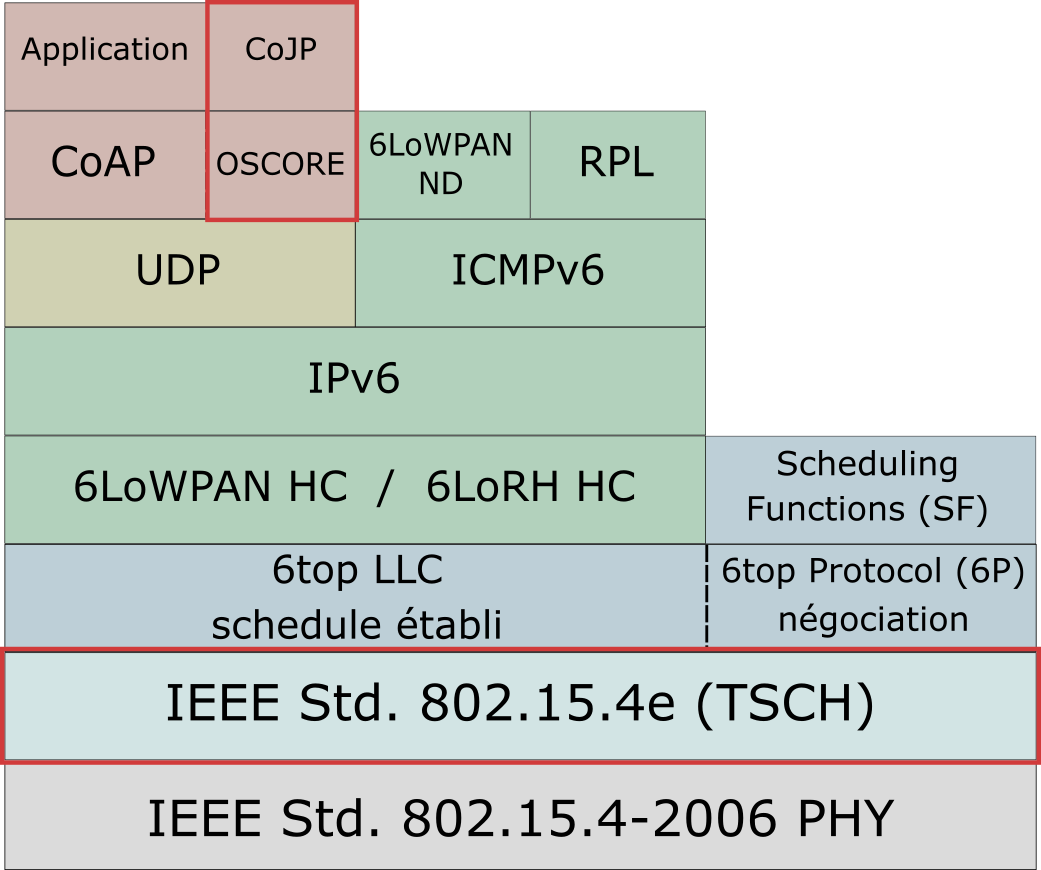
\includegraphics[width=0.6\linewidth]{6TiSCH_stack_focus}
    \caption{Pile réseau 6TiSCH}
    \end{figure}
    \end{overprint}
	}
	
    \subsection{Principes fondamentaux de TSCH}	
    
    \frame{
        \frametitle{Principes fondamentaux de TSCH}
        
        TSCH (\textit{Time Slotted Channel Hopping})
        
        Combinaison de :
        \begin{enumerate}
        \item TDMA $\rightarrow$ multiplexage en temps       (\textit{timeslot})
        \item FDMA $\rightarrow$ multiplexage en fréquences  (\textit{channelOffset})
        \end{enumerate}
        \vspace{0.5cm}
        Une communication entre nœuds voisins est caractérisée par un couple (\textit{timeslot}, \textit{channelOffset}) où
        \begin{enumerate}
        \item \textit{timeslot} donne le moment de la communication
        \item \textit{channelOffset} donne la fréquence à laquelle elle a lieu
        \end{enumerate}
        
        \vspace{0.3cm}
        
        Les nœuds communiquant possèdent et partagent cette information\\
        $\rightarrow$ communications déterministes sur base d'un \textit{schedule}
        
    }
    
    \frame{
    
    \begin{center}
            \begin{columns}[onlytextwidth,T]

        \column{5cm}	
        \centering   
    \begin{figure}
    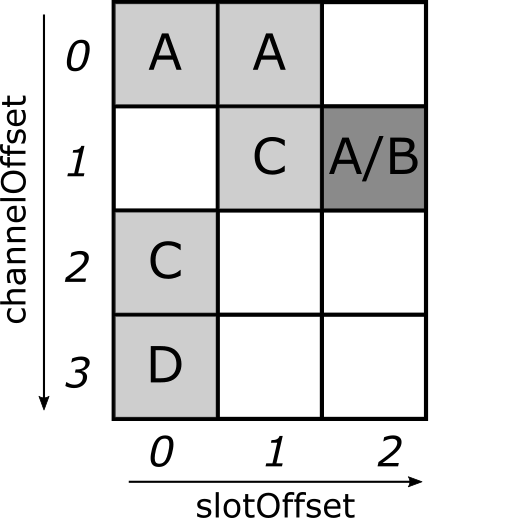
\includegraphics[width=5cm]{TSCH_basics_matrix}
    \caption{Matrice des communications}
    \end{figure}    	        
        \column{\dimexpr\linewidth-5cm}
    \begin{figure}
    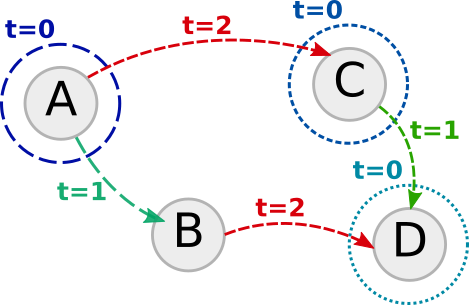
\includegraphics[width=5cm]{TSCH_basics_graph}
    \caption{Nœuds communiquant}
    \end{figure}    
	    \end{columns}
	\end{center}

    }

    \subsection{La joining phase}
    
    \frame{
        \frametitle{La joining phase}
        Réseau 6TiSCH de nœuds déjà raccordés protégé au niveau L2 par les mécanismes de protection IEEE802.15.4 et \textbf{clés} distribuées par l'autorité du réseau (\textit{\textbf{JRC}}).\\
        \vspace{0.3cm}
        Un nœud qui veut rejoindre (\textit{\textbf{pledge}}) n'a pas ces clés.\\
        \vspace{0.3cm}
        Un nœud déjà raccordé fait office de \textit{\textbf{Join Proxy}} intermédiaire entre le pledge et l'autorité du réseau.\\
\vspace{0.3cm}        
        $\rightarrow$ émission de frame spéciales (\textbf{EB}s) par les nœuds déjà raccordés\\
        \vspace{0.1cm}
        $\rightarrow$ le pledge initie la joining phase pour se synchroniser + obtenir les clés\\
        
        
    }
    
    \frame{
    \begin{figure}
    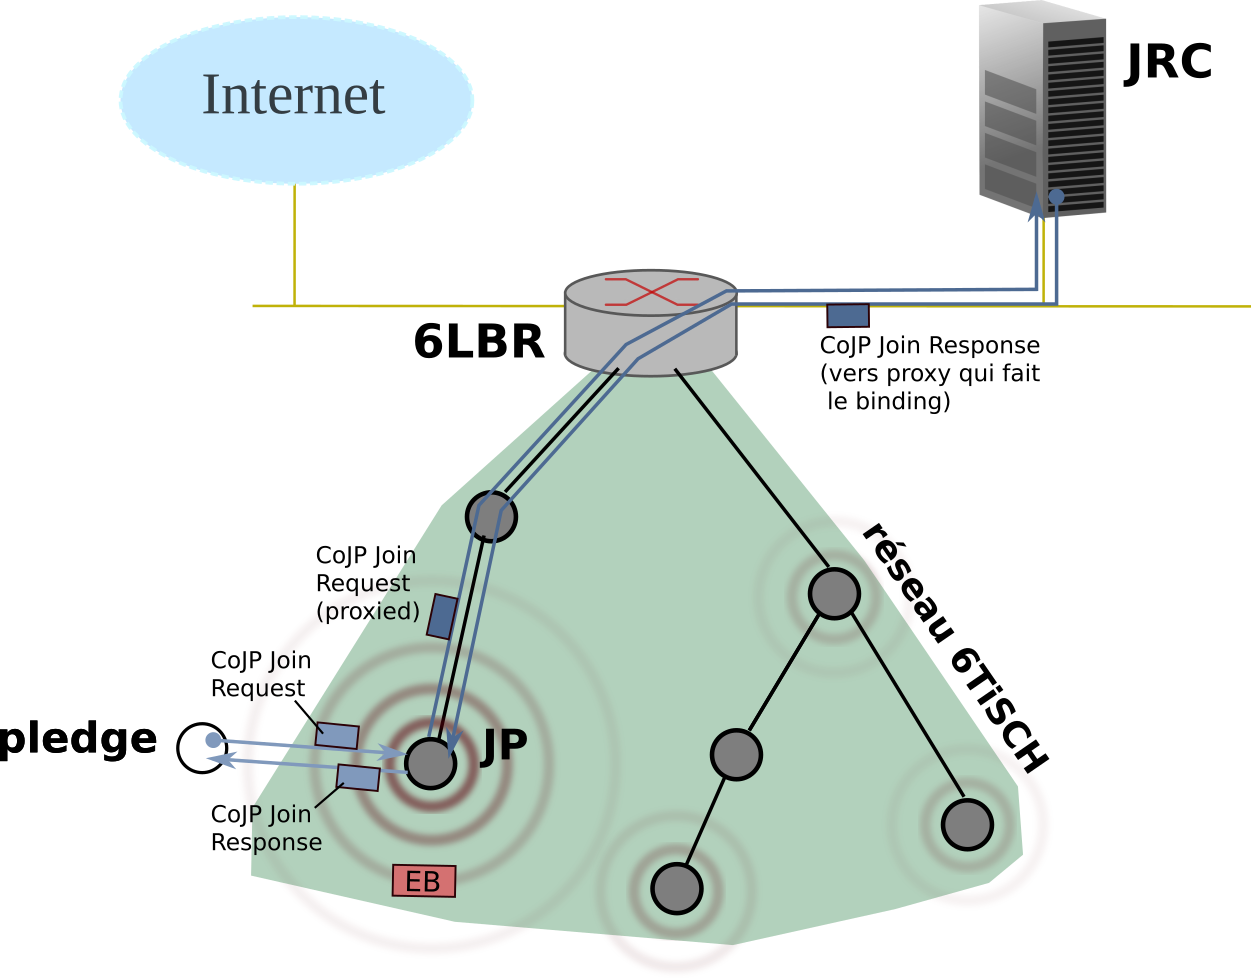
\includegraphics[width=0.75\linewidth]{Joining_phase_network}
    \caption{Join Exchange CoJP opéré lors de la joining phase d'un pledge}
    \end{figure}
    }
    
    \section{Méthode NPEB et expérimentations}
    
    \frame{
		\frametitle{Sommaire}	% Sommaire
		\tableofcontents[currentsection]
		% options = pausesections; currentsection; hideallsubsections 
	}    
    
    \subsection{Principes de la méthode NPEB}
    
    \frame{
        \frametitle{Principes de la méthode NPEB}
    
        NPEB : \textit{Neighbors propositions EB}, augmentation des EBs standards\\
        
        \vspace{0.2cm}
        Principe : un nœud annonce certains de ses voisins, proposés aux pledges qui évitent une écoute active naïve (\textbf{processus itératif d'écoute} de proposition en proposition, passe en sommeil entre).\\
        \vspace{0.4cm}
        Détermination du ``meilleur voisin" basée sur $\neq$ critères\\
        \vspace{0.5cm}
        Maintien d'une \textit{NPtable} par pledge et nœuds émettant NPEBs
        \vspace{0.2cm}
        \begin{figure}
        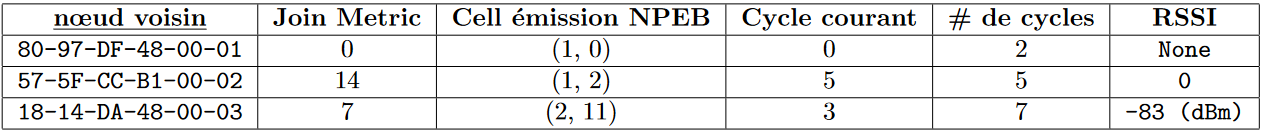
\includegraphics[width=\linewidth]{NPtable}
        \caption{Exemple de NPtable et statuts d'écoute possibles (\texttt{None}/\texttt{0}/\textit{RSSI})}
        \end{figure}
    }
    
	\frame{
	\begin{overprint}
	\onslide<1>    \begin{figure}
    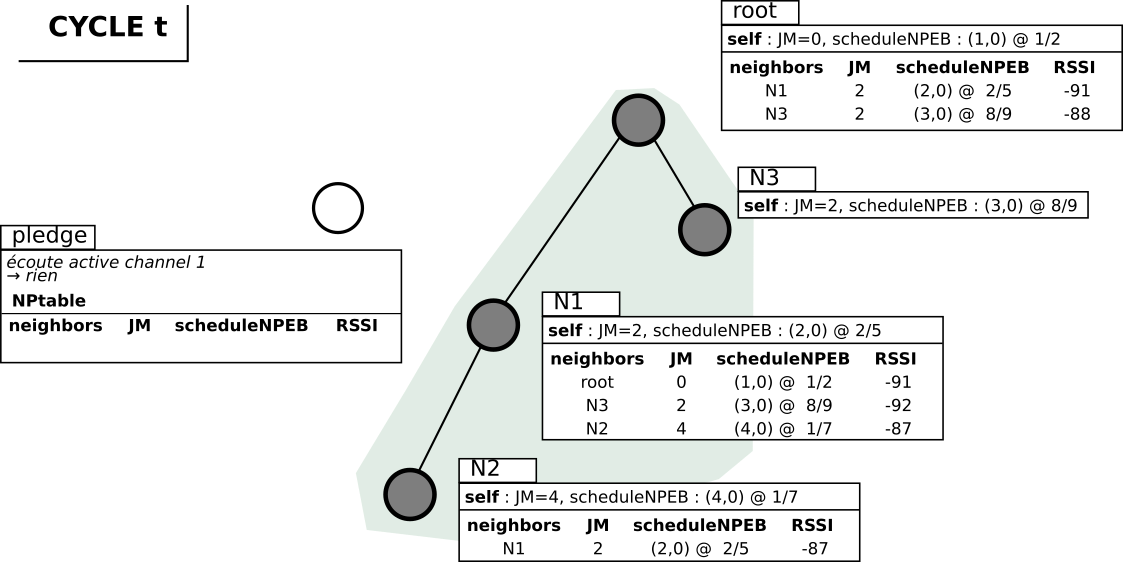
\includegraphics[width=0.85\linewidth]{NPEB_step1}
    \caption{[Cycle t] État initial du réseau où les NPtables des nœuds sont déjà alimentées}
    \end{figure}
	
	\onslide<2>    \begin{figure}
    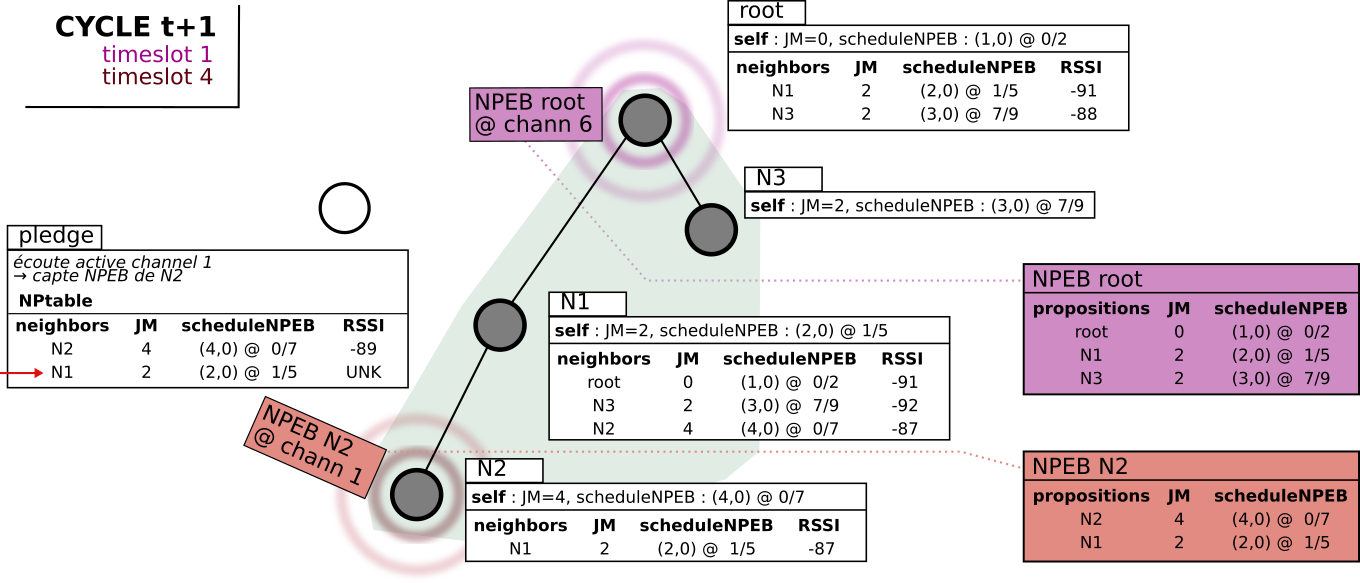
\includegraphics[width=1\linewidth]{NPEB_step2}
    \caption{[Cycle t+1] Une itération de slotframe écoulée, deux NPEBs programmés pour ce nouveau cycle}
    \end{figure}
    
    	\onslide<3>    \begin{figure}
    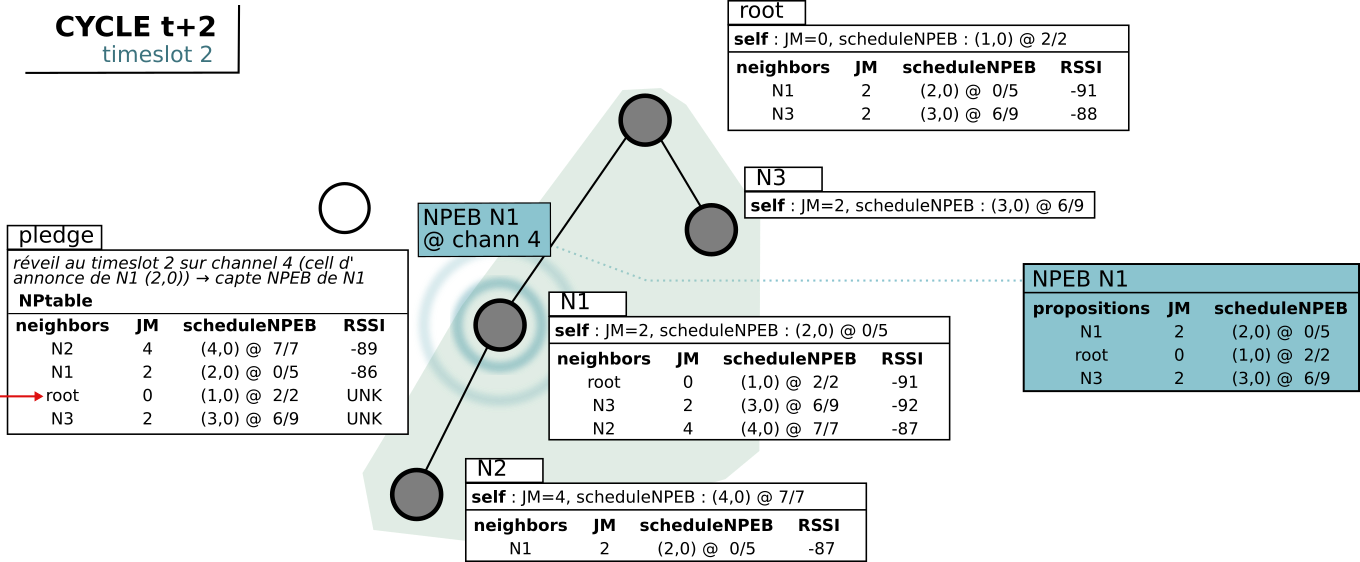
\includegraphics[width=\linewidth]{NPEB_step3}
    \caption{[Cycle t+2] sommeil du pledge jusqu'à la cell d'annonce indiquée par N1}
    \end{figure}
    
    	\onslide<4>    \begin{figure}
    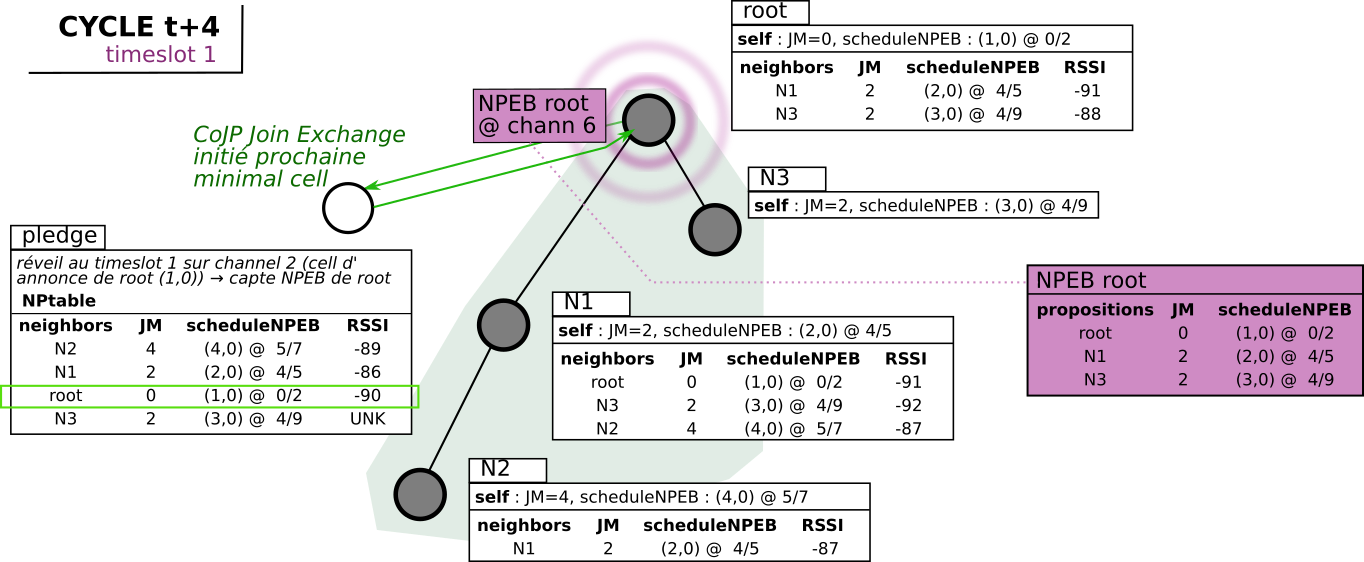
\includegraphics[width=\linewidth]{NPEB_step4}
    \caption{[Cycle t+4] sommeil du pledge jusqu'à la cell d'annonce indiquée par root et lancement de la suite du processus de join avec celui-ci}
    \end{figure}
    \end{overprint}
	}    
    
    \subsection{Évaluation de l'impact de sécurité sur la joining phase}	
	
    \frame{
        \frametitle{Impact de sécurité sur la joining phase}
        \normalsize
        Expérimentations dans le simulateur 6TiSCH :
        \begin{itemize}
        \item disposition des nœuds aléatoires
        \item $\forall$ nœud, min. 3 voisins avec PDR $>$ 50\%
        \item configuration de la pile 6TiSCH conforme aux standards
        \item même seed pour runs parallèles
        \end{itemize}
        
        \vspace{2cm}        
        
        Expérimentations : avec/sans joining phase sécurisée (i.e. Join Exchange CoJP), réseau de 10 nœuds, 20 runs
    }

    \frame{
        \begin{figure}
        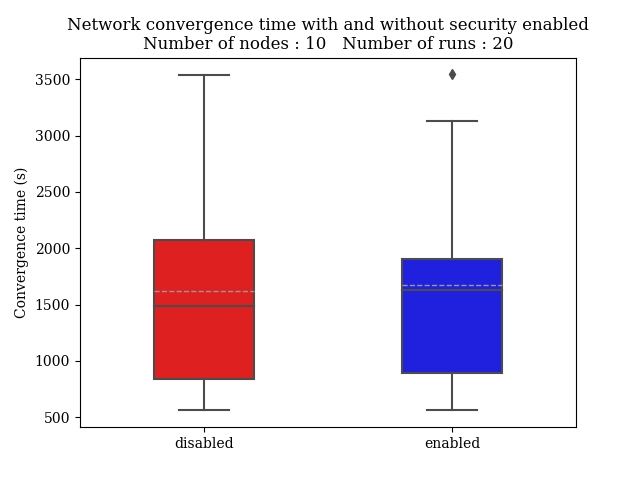
\includegraphics[width=0.75\linewidth]{{results/secjoin/boxesTimeConvergence20}}
        \caption{Temps de convergence avec/sans sécurité (Join Exchange CoJP)}
        \end{figure}
    }
    
    \frame{
        \begin{figure}
        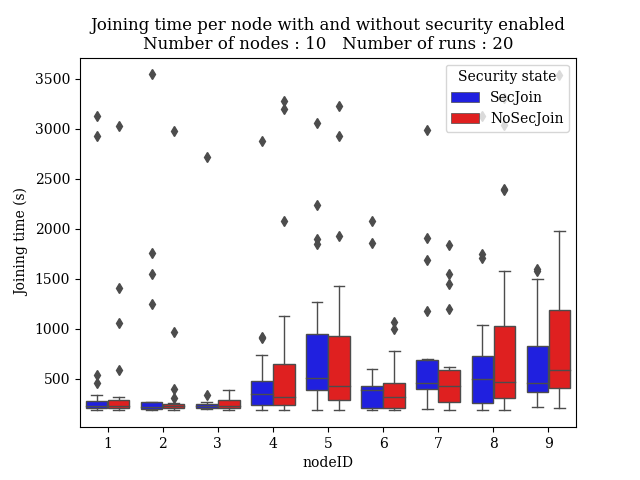
\includegraphics[width=0.75\linewidth]{{results/secjoin/boxesJoiningTimePerNode20}}
        \caption{Temps de join pour chaque nœud individuellement}
        \end{figure}
    }
    
    \frame{
        \begin{figure}
        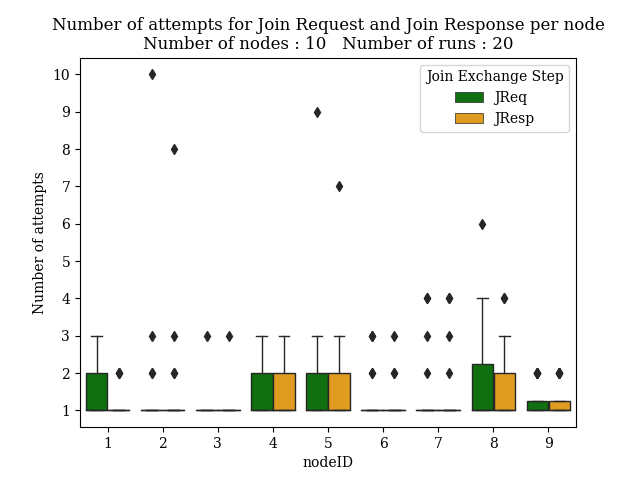
\includegraphics[width=0.75\linewidth]{{results/secjoin/boxesJoinExchange20}}
        \caption{Tentatives nécessaires pour chaque partie du Join Exchange CoJP}
        \end{figure}
    }
    
    \subsection{Évaluation des performances de la méthode NPEB}	

    \frame{
        \frametitle{Performances de la méthode NPEB}
        Intuitivement, la méthode NPEB a pour objectif de 
        \begin{enumerate}
       
        \item accélerer et optimiser en terme d'énergie (du point de vue du pledge) le processus de join
        \item permettre au pledge de sélectionner le meilleur voisin possible avec lequel initier le processus de join
        \end{enumerate}
        
        \vspace{0.3cm}
        \begin{enumerate}
        \item $\rightarrow$ division de l'analyse en fonction des étapes du processus de join, comparaison avec/sans NPEB
        \item $\rightarrow$ aucune amélioration significative, non présenté ici
        \end{enumerate}
        \vspace{0.5cm}        
        Expérimentations : avec/sans méthode NPEB implémentée dans le simulateur, réseau de 30 nœuds, 10 runs et résultats agrégés
    }
    
    \frame{
        \begin{figure}
        \includegraphics[width=0.7\linewidth]{{results/EB/phase_times}}
        \caption{[EBs] Temps requis pour $\neq$ étapes tous nœuds et runs confondus}
        \end{figure}
    }
    \frame{
        \begin{figure}
        \includegraphics[width=0.7\linewidth]{{results/NPEB/phase_times}}
        \caption{\footnotesize [NPEBs] Temps requis pour $\neq$ étapes tous nœuds et runs confondus}
        \end{figure}
    }
    
    
    \frame{
        \begin{figure}
        \includegraphics[width=0.75\linewidth]{{results/EB/phase_charges}}
        \caption{\footnotesize [EBs] Charge consommée aux $\neq$ étapes tous nœuds et runs confondus}
        \end{figure}
    }
    \frame{
        \begin{figure}
        \includegraphics[width=0.75\linewidth]{{results/NPEB/phase_charges}}
        \caption{\footnotesize [NPEBs] Charge consommée aux $\neq$ étapes tous nœuds et runs confondus}
        \end{figure}
    }
	
    \section{Conclusion}	
	
    \frame{
        \frametitle{Conclusion}
        \begin{itemize}
        \item État de l'art
        \begin{itemize}
        \item Revue de la pile dans son entièreté, conforme aux standards dans leur état actuel (standardisation toujours en cours)
        \vspace{0.1cm}
        \item Détail de la sécurité de la joining phase fait dans aucun papier publié à ce jour excepté les standards qui la décrivent eux-mêmes
        \end{itemize}
        \vspace{0.3cm}
        \item Expérimentations sur la joining phase
        \begin{itemize}
        \item Première quantification de l'impact de la sécurité sur la Joining Phase
        \vspace{0.1cm}        
        \item Élaboration de la méthode NPEB pour gagner en performances, un objectif non atteint significativement (sélection meilleur voisin)\\ $\rightarrow$ améliorations possibles par paramètres et processus décisionnels
        \end{itemize}
        \end{itemize}
    }	
	
	\frame{
	\begin{center}
	    \Large{Performances des mécanismes de sécurité du framework 6TiSCH\\}
	    \vspace{0.3cm}
	    \Huge{Q\&A}
	\vspace{0.3cm}
	   \rule{11cm}{0.6pt}\\
	\end{center}
	}
	
    \frame{
        \frametitle{Appendix}
    }	
	
    \frame{
    \centering
    $f_{eff} = HoppSeq[f \:\: \text{mod} \:\: n_{ch}]\quad$ où $f = ASN + channelOffset$
    \vspace{0.1cm}
       \begin{figure}
    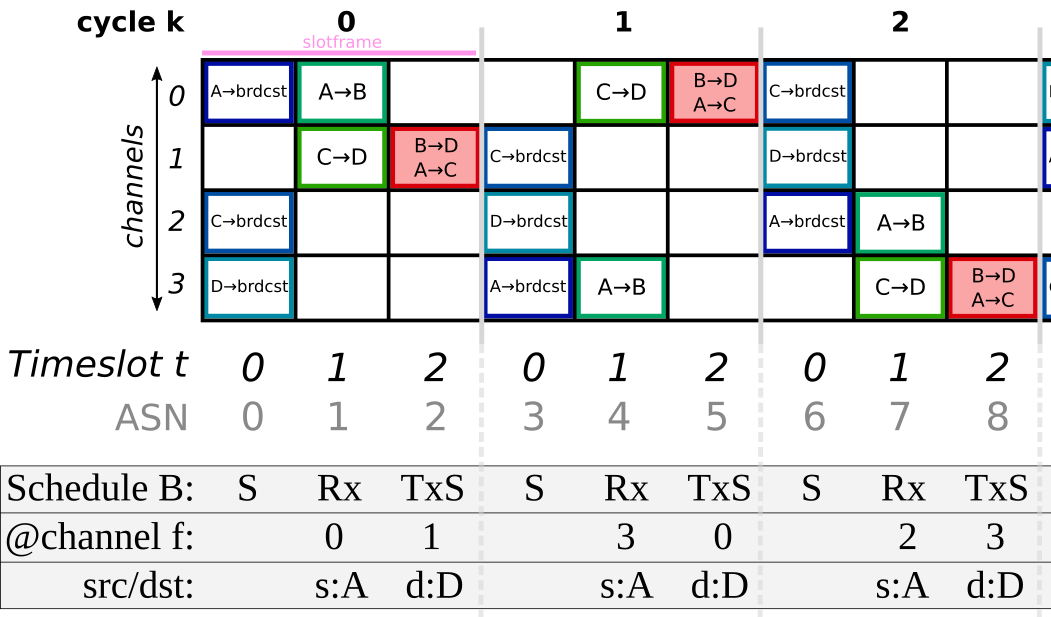
\includegraphics[width=0.8\linewidth]{TSCH_basics_schedule_croped}
    \caption{Effet de sauts de fréquence d'un cycle à l'autre de slotframe}
    \end{figure}
    }
	
\end{document}
